\documentclass[a4paper]{article}
\usepackage{lipsum}
\usepackage{tikzpagenodes}
\usepackage{pgfplots}
\usepackage{tikz}
\usepackage{tikz-3dplot}
\usetikzlibrary{arrows,decorations.pathmorphing,backgrounds,positioning,fit,matrix}
\pgfplotsset{compat=1.8}
\usepackage{graphics} % for pdf, bitmapped graphics files
\usepackage{epsfig} % for postscript graphics files
\usepackage[colorlinks=true,citecolor=green]{hyperref}
\usepackage{cite}
\usepackage{amsmath,amssymb,amsfonts}
\usepackage{algorithmic}
\usepackage{graphicx}
\usepackage{url}
\usepackage{cite}
\usepackage{bm}
\usepackage{pbox}
\usepackage{siunitx,booktabs,etoolbox}
\usepackage{ulem}

\usepackage{pgf,tikz,pgfplots}
\pgfplotsset{compat=1.15}
\usepackage{mathrsfs}

\usetikzlibrary{arrows}

\def\BibTeX{{\rm B\kern-.05em{\sc i\kern-.025em b}\kern-.08em
    T\kern-.1667em\lower.7ex\hbox{E}\kern-.125emX}}

\begin{document}
\title{Pose Estimation: $3$D to $2$D case}
\author{Xiao Hu, emails: \url{xiahaa@space.dtu.dk}}
\maketitle
\begin{figure}
\centering
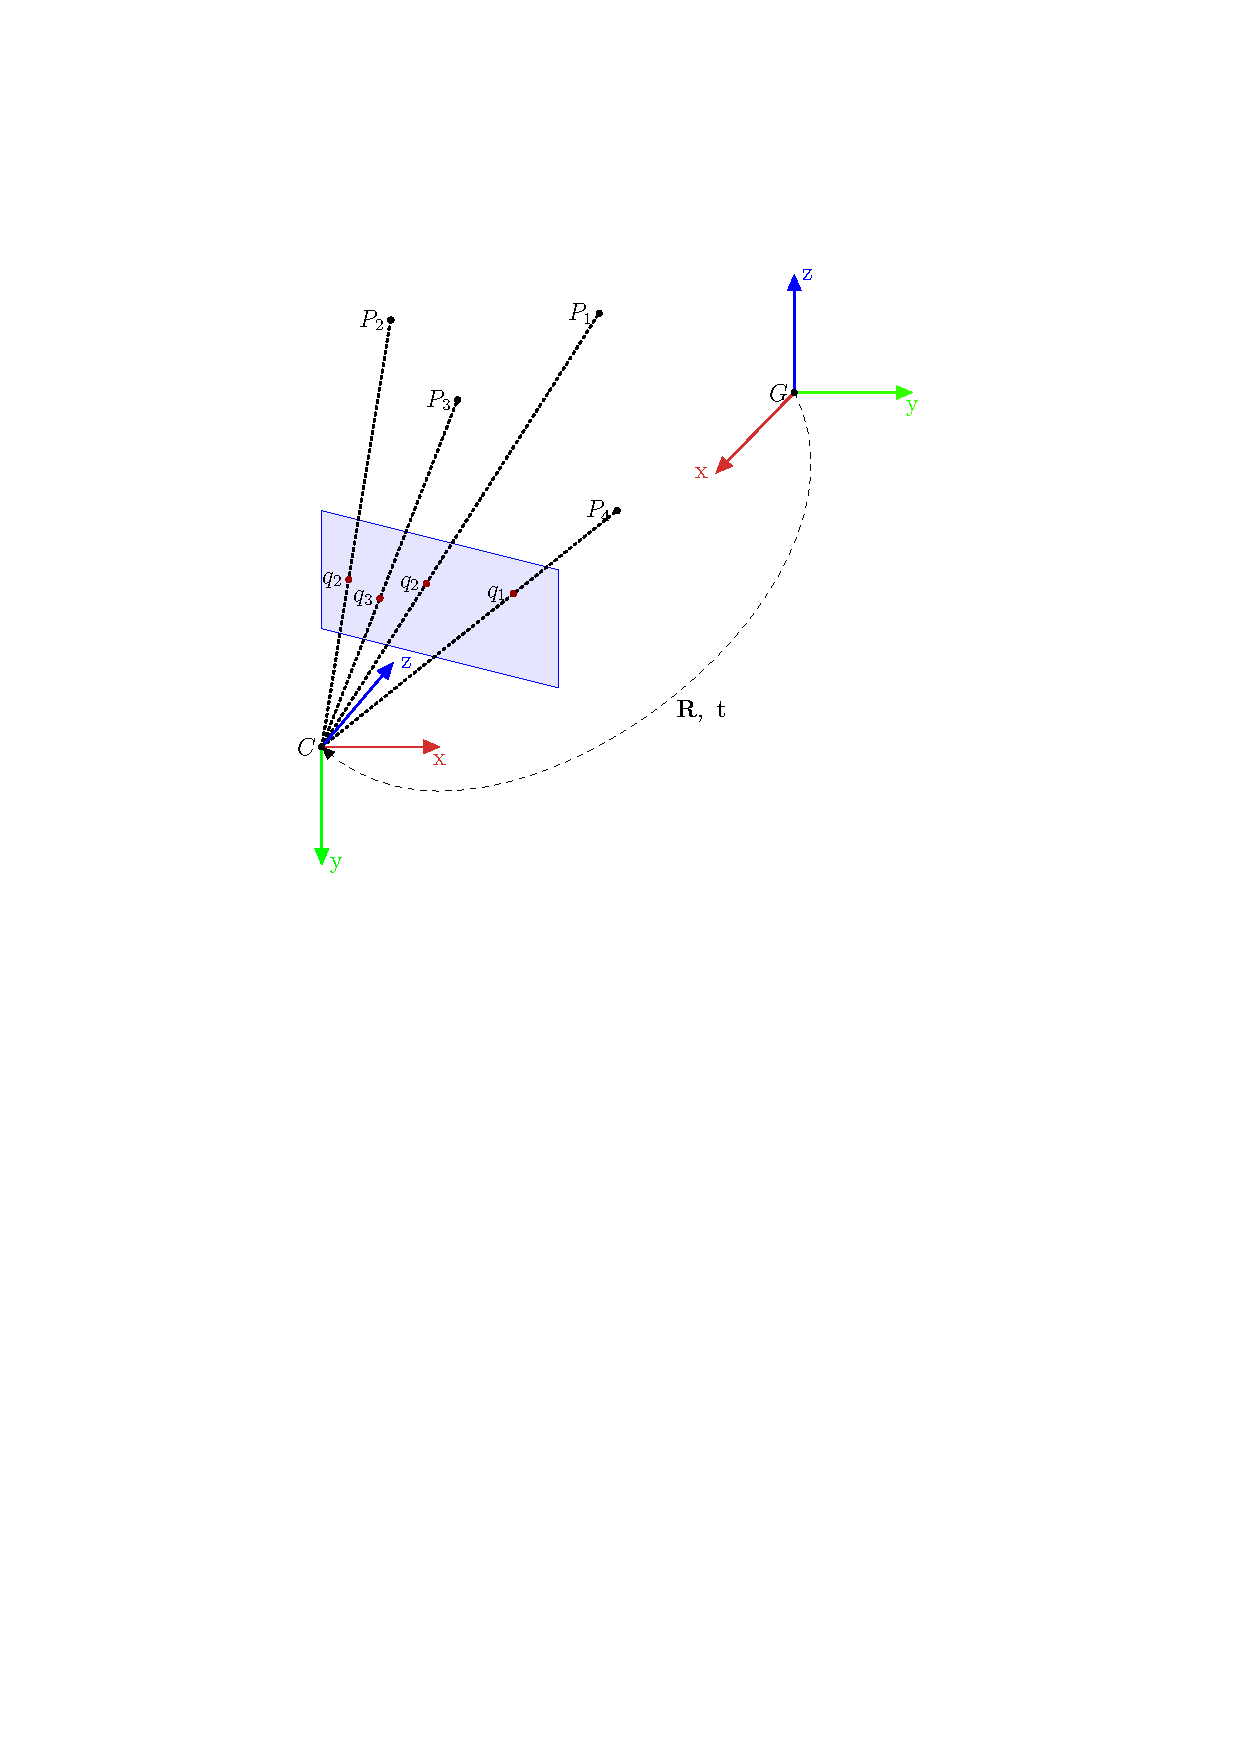
\includegraphics[scale=0.8]{hand_eye_files/vision/figures/pnp.pdf}
\caption{Principles of the Perspective $n$ Point problem.}
\end{figure}
\section{Introduction}
The Perspective-$n$-Point (P$n$P) problem is a fundamental problem in geometric computer vision. Given a certain number ($n$) of correspondences between 3D world points and 2D image measurements, the problem consists of fitting the absolute position and orientation of the camera to the measurement data~\cite{fischler1981random}. A considerable number of approaches have been proposed for the past twenty years. Generally speaking, they can be divided according to different characteristics:
\begin{itemize}
\item By whether or not the solver is run iteratively or not, Iterative V.S. Non-iterative.
\item By the require number of correspondence, P$3$P, P$4$P and more generally, P$n$P.
\end{itemize}

In my opinion, P$3$P and scalable P$n$P would be our focus since other methods are kind of intermediate products of the developing procedure. The reason why P$3$P is still favoured especially after the invention of efficient P$n$P algorithm is as follows:
\begin{itemize}
\item P$3$P is the minimal number of correspondences required to solve the general P$n$P problem. It should be noted that by adding some constraints embedded by the rigid body, this number can go down to $1$, e.g. for non-holonomic vehicle.
\item Although P$n$P algorithm can use the data redundancy to suppress the influence of noises, it can not deal with outliers. The most famous way to deal with outliers is to cascade the P$n$P algorithm with a RANSAC routine. Since for RANSAC, we prefer to use the minimal set to solve a given problem. P$3$P shows its superiority in this sense. 
\end{itemize}
The first P$3$P algorithm in a geometric view is given in~\cite{fischler1981random}, later improvements have been addressed in~\cite{pop00011},~\cite{gao2003complete}, ~\cite{li2011stable} and~\cite{kneip2011novel}.

Scalable P$n$P algorithm means the complexity of the P$n$P algorithm is $\mathcal{O}(n)$, which means its complexity or computational time grows linearly with the number of correspondence. This is very important since we would like to benefit from data redundancy without paying too much cost. The earlier P$n$P algorithms, like~\cite{ansar2003linear} ($\mathcal{O}(n^8)$) and~\cite{quan1999linear} ($\mathcal{O}(n^4)$), are not traceable if we are going to work with thousands of correspondences. EPnP~\cite{lepetit2009epnp}~\cite{moreno2007accurate} is the first P$n$P algorithm with $\mathcal{O}(n)$ complexity, followed by RPnP~\cite{li2012robust}, DLS~\cite{hesch2011direct}~\cite{nakano2015globally}, AsPnP~\cite{zheng2013aspnp}, OPnP~\cite{zheng2013revisiting}, UPnP~\cite{kneip2014upnp}.

Among iterative solutions, LHM~\cite{lu2000fast} is the most famous solution. Other solutions also exist, like RPPnP~\cite{garro2012solving} and the recently published~\cite{8470970}. Iterative solution usually show superior performance under noisy conditions. However, it is easy to see that their computational burden grows at least linearly with the number of correspondences. One of the biggest disadvantage of those iterative solutions is that the global optimality cannot be guaranteed since mathematically speaking, it is a nonlinear optimization problem which is nonconvex.

In this sense, ~\cite{schweighofer2008globally} proposed a method based on Semi-Definite Programming (SDP) and Semi-Definite Relaxation (SDR). Unfortunately, after SDR, the global optimality cannot always be retained to the original problem. Moreover, solving a SDP is usually time-consuming or at least not in real-time.

With regarding to probabilistic optimality, several methods have been proposed to solve this problem in the sense of Maximum-Likelihood Estimation (MLE)~\cite{ferraz2014leveraging},~\cite{urban2016mlpnp}. Currently, I have no plan to detail this kind of solutions. But the principle is to reformulate a cost function in order to maximize the likelihood and then solve this optimization problem iteratively. Also a reasonable estimation of the prior covariance should be built.

Planar case is one of the special case where multiple minimums can exist and hard to distinguish. Similar to~\cite{rpp}, modern approaches may provide more than one solutions if ambiguity exists. This is one point we need to be aware of. The selection of the correct result can be done with the help of other sensors or motion dynamics.

It is also worthy to mention the famous POSIT algorithm which works for object-to-image registration problem~\cite{dementhon1995model}~\cite{oberkampf1996iterative}. It is a iterative algorithm work under the assumption of weak orthogonal projection. An further improvement which allows POSIT works in unknown correspondence condition was published in~\cite{softposit}.

\textcolor{blue}{All those aforementioned algorithms have no capability of dealing with outliers themselves. RANSAC is needed in order to filter out outliers. The conventional routine for outlier removal functions like: 
\begin{itemize}
\item random select a set of correspondences.
\item apply a algorithm and testify the consensus.
\item iterate this until a certain number of iteration or inlier percentage is high enough.
\item refinement with all inliers.
\end{itemize}
This conventional routine is sometimes time-consuming since solving P$n$P and verification (usually based on reprojection error) needs to be carried out in each iteration.}
\textcolor{red}{So this is a still quite open area.} Recent work by~\cite{ferraz2014very} proposes a very fast outlier removal technique. We will detail this in the following section.

Other related topics include: solving P$n$P problem with other intrinsics unknown, such as focus length and radial distortion~\cite{pop00010}~\cite{zheng2016direct}; solving P$n$P problem with even less correspondence with the help of other constraints and sensors~\cite{pylvanainen2009revisiting},~\cite{d2014use},~\cite{d2013use}; continuous solving the P$n$P problem with observers~\cite{pop00016}; over-parameterization~\cite{pop00018}.

\section{Theory and Implementation}
There are two kind of objective functions for the P$n$P problem:

The first one is aiming to minimize the image error or the algebraic error:
\begin{align*}
f =& \underset{\mathbf{R},\ \mathbf{t}}{argmin} \sum_{i=1}^{N}||\mathbf{q}_i-\pi(\mathbf{R}\mathbf{P_i}+\mathbf{t})||^2 \Leftrightarrow \\
 &\underset{\mathbf{R},\ \mathbf{t}}{argmin} \sum_{i=1}^{N}\left((\frac{q_1}{q_3}-\frac{\mathbf{R}_(1,:)\mathbf{P_i}+t_1}{\mathbf{R}_(3,:)\mathbf{P_i}+t_3})^{2}+(\frac{q_2}{q_3}-\frac{\mathbf{R}_(2,:)\mathbf{P_i}+t_2}{\mathbf{R}_(3,:)\mathbf{P_i}+t_3})^{2}
 \right)
\end{align*}
where $\pi$ represents the projective function.

Another function is aiming to minimize the object-space error which is the alignment error of the back-tracing ray of the pixel and the ray from camera center to object points in camera coordinate frame:
\begin{align*}
f =& \underset{\mathbf{R},\ \mathbf{t}}{argmin} \sum_{i=1}^{N}||(\mathbf{I}-\mathbf{V}_i)(\mathbf{R}\mathbf{P_i}+\mathbf{t})||^2,\ with\ \mathbf{V}_i = \frac{\mathbf{q_iq_i}^T}{\mathbf{q_i}^T\mathbf{q_i}}
\end{align*}
\textbf{Note:} we assume here $\mathbf{q}_i$ has been normalized ($\mathbf{q}_i = \mathbf{K}^{-1}\mathbf{q}_i'$).

Generally speaking, the P$n$P problem is to find the answer for the aforementioned two optimization problem. What makes this problem challenging is the rotation matrix $\mathbf{R}\in \mathbb{SO}(3)$ which will implicitly impose nonlinear, nonconvex constraints. This is why the famous Direct-Linear-Transformation (DLT)\footnote{DLT means we omit those constraints and take each elements of $\mathbf{R}$ as separate variables. This can make the objective function as well as the constraints in affine or quadratic form.} method cannot given us a promising result.

Here are some useful techniques which will help us solve this problem~\cite{hartley2007optimal}:
\begin{itemize}
\item Branch-and-Bounding;
\item Convex optimization, such as Second-Order-Cone-Programming (SOCP), SDP: this usually requires relaxation or even solve the prime problem by solving the dual problem;
\item Algebraic Geometry: use Gr\"{o}ebner basis. This is feasible since the objective function and the constraints can be formulate as a polynomial system and the answer is the common root that makes those polynomials vanish~\cite{kukelova2008automatic}. 
\item Manifold Optimization which applies optimization directly on $\mathbb{SO}(3)$ and $\mathbb{SE}(3)$.
\end{itemize}

\subsection{P$3$P}
We start with the P$3$P algorithms. Generally speaking, the P$3$P problem solves this problem by firstly estimating the arc-length of each points in the camera frame, then reconstructs the point cloud in the camera frame by multiplying the arc-length with the back-tracing rays, and finally applies the $3$D to $3$D pose estimation routines in order to find the $\mathbf{R}$ and $\mathbf{t}$.
\begin{figure}
\centering
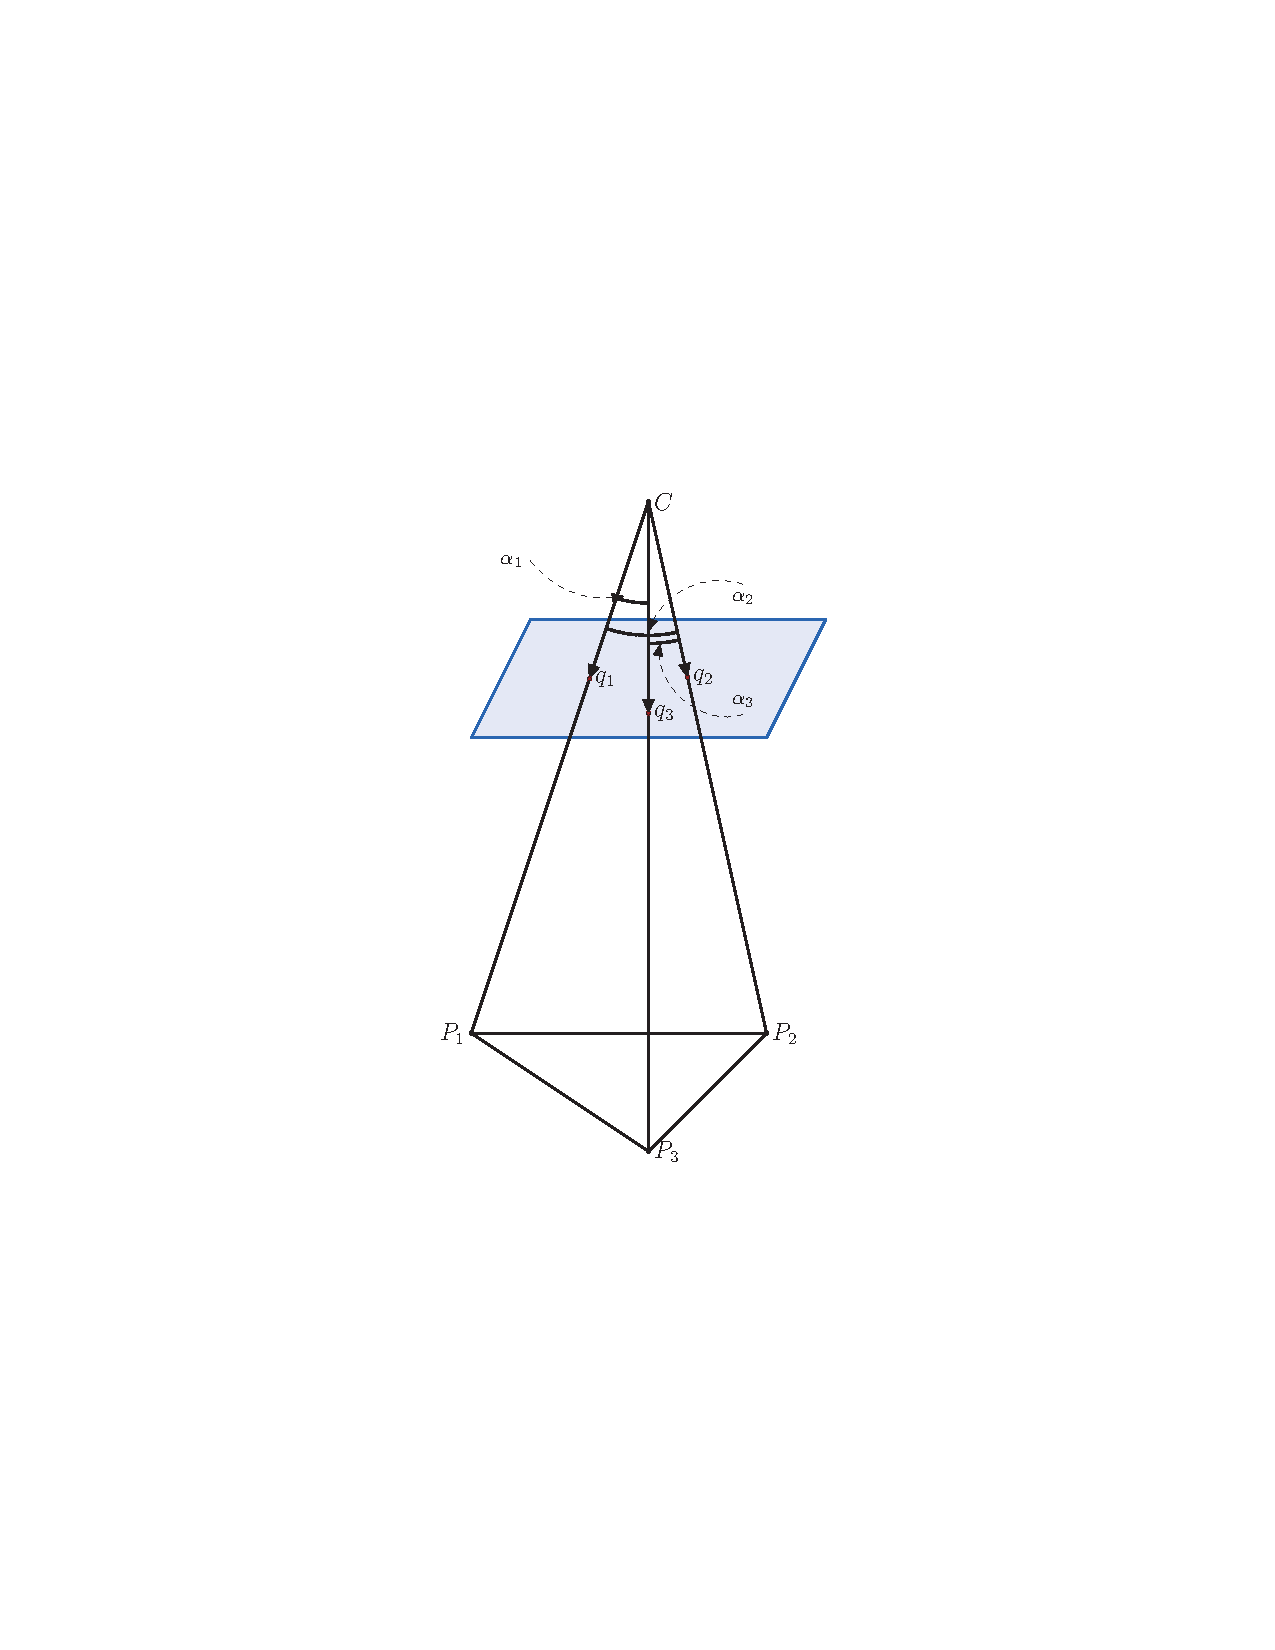
\includegraphics[scale=0.8]{hand_eye_files/vision/figures/p3p.pdf}
\caption{Principles of the Perspective $3$ Point problem.}
\label{fig:p3p}
\end{figure}
\begin{figure}
\centering
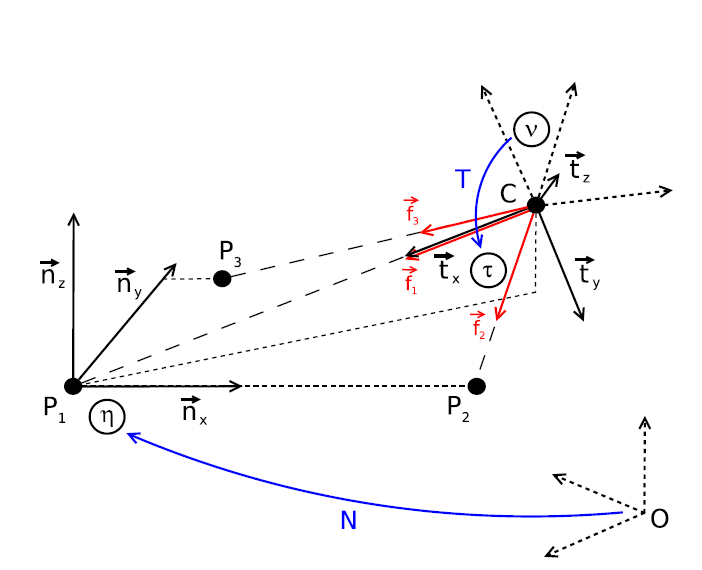
\includegraphics[scale=0.5]{hand_eye_files/vision/figures/p3p_kneip.png}
\caption{Figure from~\cite{kneip2011novel}.}
\label{fig:p3p}
\end{figure}
From Fig~\ref{fig:p3p}, by denoting $|CP_1|=d1,\ |CP_2|=d2,\ |CP_3|=d3,\ |P_1P_2|=d12,\ |P_1P_3|=d13,\ |P_2P_3|=d23,\ $, we will have the following relationship using the cosine rule:
\begin{align*}
d12^2 = d1^2+d2^2-2cos(\alpha_2)d1d2 \\
d13^2 = d1^2+d3^2-2cos(\alpha_1)d1d3 \\
d23^2 = d2^2+d3^2-2cos(\alpha_3)d2d3 \\
\end{align*}
where $\alpha_1 = acos(\mathbf{q}_1 \cdot \mathbf{q}_3),\ \alpha_2 = acos(\mathbf{q}_1 \cdot \mathbf{q}_2),\ \alpha_3 = acos(\mathbf{q}_2 \cdot \mathbf{q}_3)$. By some algebraic operations\footnote{eliminate one variable by the other two and then continue}, we will have a $4^{th}$ order polynomial equation:
\begin{align*}
A_4 t^4+A_3 t^3+A_2 t^2+A_1 t^1+A_0 = 0
\end{align*}
By solving this equation, we will have the arc-length. Continue this for other arcs, we can find them all. By multiplying $\mathbf{q}_i$ with $d_i$, we will have $\mathbf{Q}_i$, then the problem transforms to:
\begin{align*}
f =& \underset{\mathbf{R},\ \mathbf{t}}{argmin} \sum_{i=1}^{N}||\mathbf{Q}_i-\mathbf{R}\mathbf{P_i}+\mathbf{t}||^2
\end{align*}
which is a typical $3$D to $3$D pose estimation problem that can be solved.

P$3$P methods~\cite{fischler1981random},~\cite{gao2003complete}, and~\cite{li2011stable} all function in this way. ~\cite{fischler1981random} is more like a hard-code solution.~\cite{gao2003complete} gives detailed illustration of the P$3$P problem and also their solution under some degenerate cases. However,~\cite{gao2003complete} is too mathematical which is hard to read. But if you only care about the solution, then you can go directly to the normal case.~\cite{li2011stable} is the most clear paper that clearly explain this problem.


The only different P$3$P method was proposed in~\cite{kneip2011novel}. By introducing two intermediate frames, it changes the original $3$D to $2$D problem to a plane problem. After geometric operations, it finally results in a $4^{th}$ order polynomial equation. However, this $4^{th}$ order polynomial does not take arc-length as the variable, but an alternative parameter which represent the tilt angle of the $P_1-P_2-C$ plane. So the final $\mathbf{R},\ \mathbf{t}$ have to be found in another way rather than solving the $3$D to $3$D pose estimation problem. \textcolor{blue}{This method is easy to understand and very fast.}

\subsubsection{Summary of P$3$P}
Here are several points which remains unclear:
\begin{itemize}
\item which P$3$P gives the best performance in terms of stability, runtime?
\item how can P$3$P benefit from data redundancy? Or P$3$P can only be used for outlier removal together with RANSAC?
\end{itemize}

\subsection{Complex P$n$P}
Here, Complex P$n$P means not-well scalable P$n$P algorithms such as~\cite{quan1999linear} and~\cite{ansar2003linear}. I will begin with~\cite{quan1999linear} and then talk about~\cite{ansar2003linear}.

The linear P$n$P in~\cite{quan1999linear} is based on the cosine rule function we have seen in P$3$P.~\cite{quan1999linear} uses the Sylvester resultant to eliminate variable, which will result in a $8^{th}$ order polynomial which only contains even terms (equals to a $4^{th}$ order polynomial). The idea is quite straightforward: since each tuple-3, e.g ${1,2,3} or {1,4,5}$, will generate a $4^{th}$ order polynomial in, e.g. $d_1$. So, $N$ points generates $C_{N}^{2}$ cosine equations which furthermore generates $\frac{(n-1)(n-2)}{2}$ $4^{th}$ order polynomials (eliminating redundant polynomials). By taking the linearization which means taking $\mathbf{t}=(1,x,x^2,x^3,x^4)^{T}$ as separate terms, we will have a equation like $\mathbf{A}\mathbf{t}=0$. 
$$
\underbrace{
\left[
\begin{matrix}
\mathbf{a}_1 \\
\mathbf{a}_2 \\
\vdots \\
\mathbf{a}_K \\
\end{matrix}
\right]}_{\mathbf{A}}
\left[
\begin{matrix}
1 \\ x \\ x^2 \\ x^3 \\ x^4
\end{matrix}
\right]=\mathbf{0}
$$
Then $\mathbf{t}$ can be found by taking the right singular vector. Supposing the dimension of the null space is over one, which means 
$$
x = \lambda \mathbf{v}_4 + \beta \mathbf{v}_5, \lambda, \beta \in \mathbb{R}.
$$
In order to solve for $\lambda, \beta$, we should use the so-called re-linearization technique:
Notice that $t_it_j=t_kt_l,\ if\ i+j=k+l$, so we call formulate another normal system with $(\lambda^2, \lambda\beta, \beta^2$. We solve again for $\lambda, \beta$ and then for $d_i$. The final pose estimation problem, once again, turns out to be a $3$D to $3$D pose estimation problem. \textcolor{blue}{As can be seen from here, data redundancy is utilized by stacking the $4^{th}$ order polynomial equation and find the null vector. However, since the aforementioned procedure has to be run for each possible arc, for sure, the complexity does not scale very well.}

Another linear P$n$P algorithm is proposed in~\cite{ansar2003linear}. It also starts with the cosine equations. However, they applied linearization as follows:
\begin{align*}
&\text{recall: } x_1^2+x^2-2x_1x_2cos(\alpha_{12})-d_{12}^2=0 \\
&\text{linearization: $\mathbf{t}={x_1^2, x_1x_2, x_2^2}$} \\
&\text{do this for $N$} \Leftrightarrow \\
&\underbrace{
\left[
\begin{matrix}
-2cos(\alpha_{12}) & 0 & \cdots & 0 \\
0 & -2cos(\alpha_{13}) & \cdots & 0 \\
\vdots & \vdots & \ddots & \vdots \\
0 & 0 & \cdots & -2cos(\alpha_{n, n-1})\\
\end{matrix}
\right.
\left|
\begin{matrix}
1 & 1 & 0 & \cdots & 0 & 0 & -d_{12}^2\\
1 & 0 & 1 & \cdots & 0 & 0 & -d_{13}^2\\
\vdots & \vdots & \vdots& \ddots & \ddots & vdots & vdots \\
0 & 0 & \cdots & cdots & 1 & 1 & -d_{n, n-1}^2\\
\end{matrix}
\right]
}_{\mathbf{M}} \\
&\mathbf{M}\mathbf{t} = \mathbf{0}
\end{align*}
Finding $\mathbf{t}$ by choosing the rightmost singular vector and apply a similar relinearization to recover $x$. For $N$ points, we have $C_{N}^2$ cosine equations. Then we have $N$ terms in form of $x_i^2$, $C_{N}^2$ terms in form of $x_ix_j$ and one slack variable $1$. So in total, the solution vector is $\frac{N(N+1)}{2}+1$. The kernel is of dimension $\frac{N(N-1)}{2}$, so we will have a null space of dimension $N+1$. We still needs $\frac{N*N*(N-1)}{2}$ constraints to do the relinearization. As can be seen, this method is extremely complex. The computation time will increase significantly with the number of correspondences. \textcolor{red}{This method is only theoretically meaningful, but cannot be used in practice, especially now we have the $\mathcal{O}(n)$ solutions.}


\bibliography{PnPCites} 
\bibliographystyle{ieeetr}

\end{document}